\documentclass{beamer}
\usepackage[utf8]{inputenc}
\usepackage{xeCJK}
\usepackage{graphicx}
\usepackage{amsmath}

\setCJKmainfont{PingFang TC}

\title{哥布林介紹}
\author{作者名稱}
\date{\today}

\begin{document}

\begin{frame}
    \titlepage
\end{frame}

\begin{frame}{目錄}
    \tableofcontents
\end{frame}

\section{Perceptron}
% 第一頁:Perceptron 介紹
\begin{frame}{Perceptron 簡介}
\begin{itemize}
  \item 1958 年由 Frank Rosenblatt 提出,為早期生物啟發的神經網路模型  
  \item 改進 McCulloch–Pitts 模型,加入\alert{可更新的權重}與\alert{錯誤修正學習}  
  \item 可解決\textbf{線性可分}之二分類問題(例如:貓 vs 狗)  
  \item 三層結構:輸入層(感官)→ 聯想層(隱藏)→ 輸出層(回饋學習)  
  \item 核心機制:\textbf{誤差更正(error-correction learning)}:contentReference[oaicite:0]{index=0}
\end{itemize}
\end{frame}

% 第二頁:Perceptron 的數學原理
\begin{frame}{Perceptron 的數學原理}
\begin{enumerate}
  \item \textbf{線性加權總和}
  \[
    z = \sum_{i=1}^{n} w_i x_i + b
  \]
  \item \textbf{階梯啟動函數(Threshold)}
  \[
    \hat{y} =
    \begin{cases}
      +1, & z \ge 0,\\
      -1, & z < 0.
    \end{cases}
  \]
  \item \textbf{權重更新規則(Error-Correction)}
  \[
    w_i \leftarrow w_i + \eta\,\bigl(y - \hat{y}\bigr)\,x_i,
    \quad
    b \leftarrow b + \eta\,(y - \hat{y})
  \]
  \begin{itemize}
    \item $\eta$:學習率,決定單次更新的步幅  
    \item 保證\textbf{線性可分問題}下收斂至正確分類:contentReference[oaicite:1]{index=1}
  \end{itemize}
\end{enumerate}
\end{frame}

\begin{frame}{ADALINE 自適應線性神經元}
    \begin{center}
        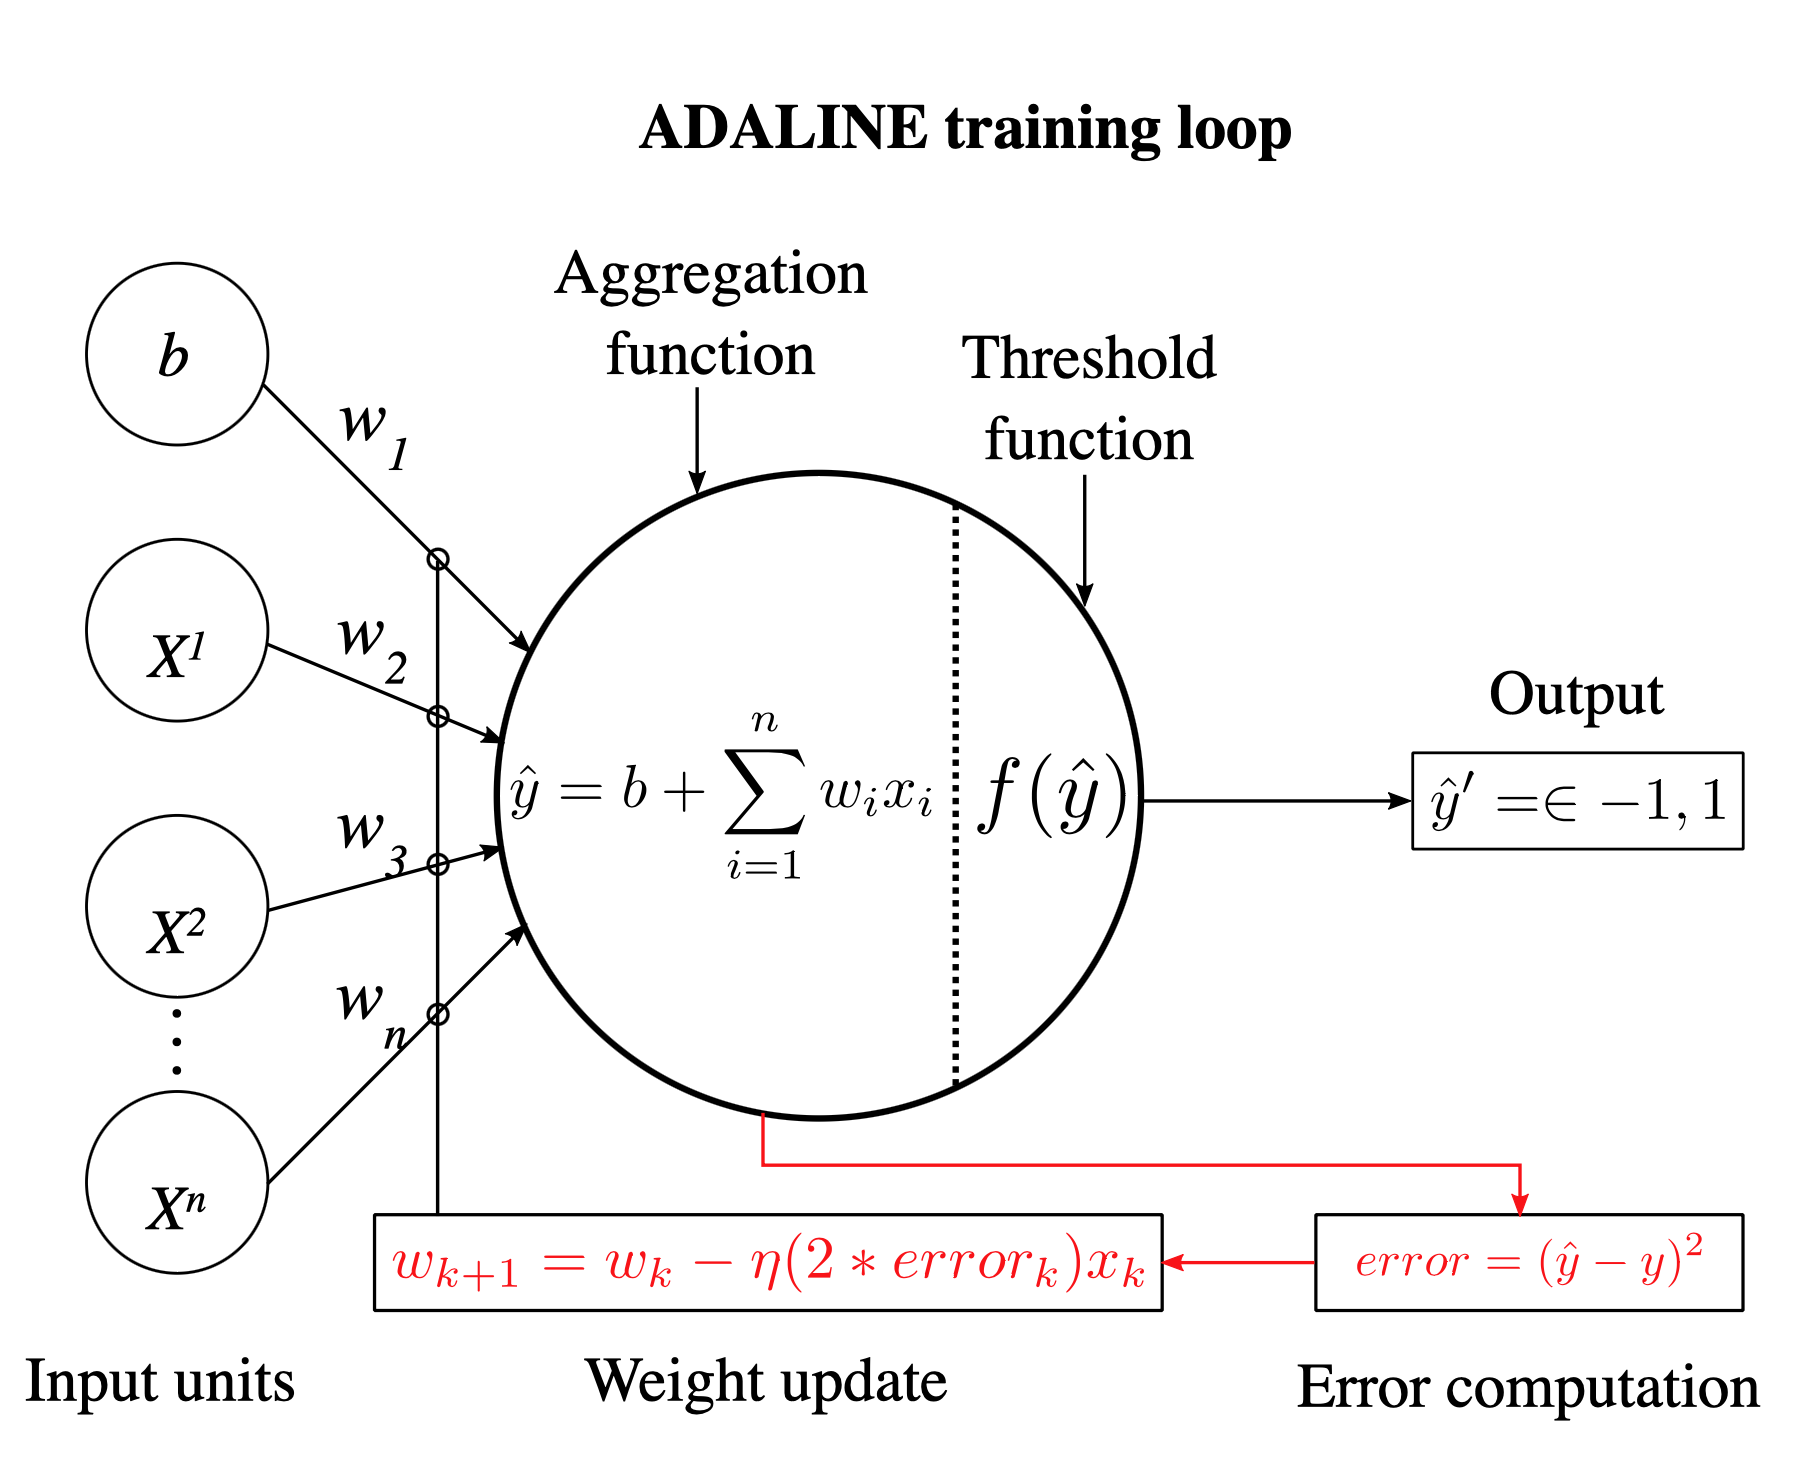
\includegraphics[width=0.8\textwidth]{ADALINE_picture.png}
    \end{center}
\end{frame}

% 概覽
\begin{frame}{Overview}
\begin{itemize}
\item 發明者:Widrow \& Hoff (1959)
\item 目標:最小化均方誤差 (MSE)
\item 特點:線性輸出,連續可微
\item 演算法:Gradient Descent
\item 優勢:收斂穩定、更新平滑
\end{itemize}
\end{frame}

% 數學形式
\begin{frame}{ADALINE 數學形式}
\[
  \hat y = \mathbf{w}^\top \mathbf{x} + b
\]
\[
  \mathrm{MSE} = \frac{1}{n}\sum_{i=1}^n(y_i - \hat y_i)^2
\]
\[
  w \leftarrow w - \eta\,(y - \hat y)\,x
\]
\end{frame}

% 訓練演算法
\begin{frame}{訓練演算法}
\begin{itemize}
\item 計算 linear aggregation: $\hat y$
\item 計算 error: $(y - \hat y)^2$
\item 更新權重: $w \leftarrow w - \eta\,(y - \hat y)x$
\end{itemize}
\end{frame}

% 應用場景
\begin{frame}{應用場景}
\begin{itemize}
\item 自適應濾波 (Adaptive Filtering)
\item 噪音消除 (Noise Cancellation)
\item 時序預測 (Time Series Prediction)
\item 自動控制系統 (Control Systems)
\end{itemize}
\end{frame}

\section{哥布林的特徵}
\begin{frame}{哥布林的特徵}
    \begin{itemize}
        \item 身材矮小,皮膚多為綠色或灰色。
        \item 通常有尖耳朵、大鼻子、銳利的牙齒。
        \item 性格狡猾、貪婪,有時帶點幽默感。
    \end{itemize}
\end{frame}

\section{哥布林在文化中的形象}
\begin{frame}{哥布林在文化中的形象}
    \begin{itemize}
        \item 在《魔戒》、《哈利波特》等作品中都有出現。
        \item 遊戲如《魔獸世界》、《龍與地下城》也有各種哥布林角色。
    \end{itemize}
\end{frame}

\section{哥布林的數學趣談}
\begin{frame}{哥布林的數學趣談}
    假設有 5 個哥布林要分 20 枚金幣,每個哥布林至少要分到 2 枚,請問有多少種分法?
    \[
    \text{這是一個經典的整數分拆問題。}
    \]
\end{frame}

\end{document} 